\documentclass[10pt,letterpaper]{article}

\usepackage{fontspec}
\setmainfont{texgyretermes-regular.otf}[BoldFont=texgyretermes-bold.otf,ItalicFont=texgyretermes-italic.otf,BoldItalicFont=texgyretermes-bolditalic.otf]
\usepackage{unicode-math}
\setmathfont{texgyretermes-math.otf}

\usepackage[letterpaper,margin=1in]{geometry}
\usepackage{amsmath}
\usepackage{graphicx}
\usepackage{booktabs}
\usepackage{array}
\usepackage{tabularx}
\usepackage[font=small,labelfont=bf,justification=raggedright,singlelinecheck=false]{caption}
\usepackage{microtype}
\usepackage[hidelinks]{hyperref}
\hypersetup{
  pdftitle={The x16 Ceiling: Connector, Silicon, and Latency Constraints on Memory Bandwidth over PCI Express},
  pdfauthor={Amrendra Singh and DeepSeek V4.1 Flash 1017},
  pdfsubject={PCI Express, memory bandwidth, CXL, interconnect},
  pdfkeywords={PCIe, CXL, memory bandwidth, SerDes, interconnect}
}
\usepackage{titlesec}

\graphicspath{{../figures/}}

\setlength{\parindent}{1.2em}
\setlength{\parskip}{0pt}
\emergencystretch=1em

\titleformat{\section}{\large\bfseries}{\thesection.}{0.5em}{}
\titleformat{\subsection}{\normalsize\bfseries}{\thesubsection}{0.5em}{}
\titlespacing*{\section}{0pt}{1.5ex plus .3ex}{0.6ex}
\titlespacing*{\subsection}{0pt}{1.2ex plus .2ex}{0.3ex}

\begin{document}

\title{\textsc{\small Technical Report $\cdot$ Draft}\\[10pt]
\textbf{The x16 Ceiling}\\[5pt]
{\large Connector, Silicon, and Latency Constraints on Memory Bandwidth over PCI Express}}
\author{\normalsize Amrendra Singh and DeepSeek V4.1 Flash 1017}
\date{\normalsize 2026}
\maketitle
\vspace{-1.4em}

\begin{abstract}
\noindent PCI Express has carried memory traffic for two decades. Its per-lane rate has grown fifty-fold and its x16 bandwidth sixty-fold, yet its width has not moved: every generation still terminates at sixteen lanes and a 164-pin edge connector. This paper argues that the bandwidth of memory reached through PCIe is set less by signaling rate than by three rations the standard never lifted---a pin ration at the connector, an area-and-power ration in the SerDes and root complex, and a transaction ration that forces memory traffic into small payloads and a finite tag space. We quantify each budget and combine them in a model whose effective bandwidth is the minimum of a link ceiling and a latency bound, $B_{\mathrm{eff}} = \min(B_{\mathrm{link}}\eta,\, NP/\mathrm{RTT})$. The model shows that a single PCIe function's 256-tag space caps cache-line throughput at roughly 16~GB/s at one microsecond of round-trip latency, well below a Gen5 x16 link; that 64-byte payloads waste about a quarter of the link on headers; and that, per signal pin, PCIe Gen6 and Gen7 now exceed HBM3E, so the gap between the two is a matter of pin count and reach rather than signaling. We use the model to compare CXL, NVLink/UALink, optical links, and UCIe by which ration each relaxes, and conclude that the next decade of memory bandwidth will be won by adding pins and shortening reach, not by raising frequency.
\end{abstract}

\noindent\textbf{Keywords:} PCI Express; memory bandwidth; CXL; SerDes; interconnect; memory wall.

\section{Introduction}

An accelerator today reads its own memory at three to eight terabytes per second and its host's memory at sixty-three gigabytes per second over a Gen5 x16 link. The ratio---fifty to a hundred---is the most consequential number in system architecture after the arithmetic intensity of the workload itself. Every model that does not fit in device memory, every key-value cache that spills, every checkpoint, and every gradient that leaves the rack crosses that ratio.

Wulf and McKee named the processor--DRAM gap the memory wall in 1995 \cite{wulf}. Three decades later the wall has moved rather than disappeared: the fast memory is now the accelerator's HBM, the slow memory is everything reachable over an I/O interconnect, and the interconnect is almost always PCI Express. At rack scale the same logic applies to the datacenter as a whole, which is increasingly a memory hierarchy with processors attached \cite{barroso}. The accelerator itself is the proof that bandwidth, not arithmetic, is the scarce resource: the tensor processors that made deep learning practical were designed around a memory system, and their successors are designed around a memory system that is an order of magnitude larger \cite{jouppi}.

By the standard's own metric, PCIe is a triumph. Per-lane signaling has risen from 2.5 to 128~GT/s; x16 bandwidth has risen from 4~GB/s to 242~GB/s, a sixty-fold gain delivered almost entirely by better equalization, modulation, and coding \cite{pcie6,pcie7}. By the system designer's metric, something else has been frozen. The x16 edge connector of 2003 and the x16 edge connector of 2025 both present 64 high-speed pins. The protocol permits wider links; the connector does not.

The industry markets generations in gigatransfers. A system experiences pins, reach, and latency. This paper argues that the bandwidth of memory reached through PCIe is governed by three rations that the standard has never lifted: a pin ration at the connector, an area-and-power ration in the SerDes and root complex, and a transaction ration that forces memory traffic into small payloads and a finite tag space. Each is a budget. The smallest one binds, and for cache-line memory traffic it is usually not the link rate.

Our contributions are four. First, we give a quantitative account of the connector and silicon budgets, with the numbers that a system designer can check (Sections~\ref{sec:connector} and~\ref{sec:silicon}). Second, we combine link rate, protocol efficiency, and outstanding-request limits in a latency-bound model and show where each term binds (Section~\ref{sec:model}). Third, we reframe the HBM--PCIe gap as a pin-count and reach problem rather than a signaling problem, using a per-pin comparison that puts PCIe Gen6 ahead of HBM3E (Section~\ref{sec:perpin}). Fourth, we map CXL, NVLink/UALink, optics, and UCIe to the specific ration each relaxes, and argue that the next decade of memory bandwidth is a packaging problem (Section~\ref{sec:escape}).

Our method is analytical. We take rates, widths, and overheads from the public specifications and published architecture descriptions, and we build a first-order model rather than a calibrated simulator. The parameters are listed in Table~\ref{tab:budgets} so that a reader can substitute their own. We do not report measurements, and we flag estimates as estimates.

\section{Background: PCIe as a Memory Transport}

\subsection{The transaction model}

PCIe is a layered, packetized, split-transaction interconnect. A memory read is a non-posted request that returns one or more completions; a write is posted. Transaction-layer packets carry 12- or 16-byte headers, a payload of 128 to 4096 bytes, and an optional ECRC. The data-link layer adds a sequence number and a link CRC; the physical layer encodes the result. Because reads are split, a requester must keep multiple requests in flight to cover the round trip, and the number it can keep in flight is bounded by the Tag field: five bits by default, eight with Extended Tag Enable, for 32 or 256 outstanding requests per function \cite{pcie6}. Phantom functions can extend this several-fold, at the cost of complexity.

Gen6 changed the framing. It moved to PAM4 at 64~GT/s, replaced variable-length framing with fixed 256-byte flits, and added a lightweight forward error correction, so the link is more robust but also more structured; Gen7 doubles the rate to 128~GT/s on the same model \cite{pcie6,pcie7}. The important continuity is that the transaction layer still moves memory in packets whose header-to-payload ratio is set by the cache line, not by the link.

\subsection{Generations and encoding}

Table~\ref{tab:gens} and Figure~\ref{fig:scaling} summarize the seven generations. The table separates raw signaling from usable bandwidth, because the two are frequently conflated in product literature.

\begin{table}[t]
\centering
\caption{PCIe generations, one direction. Usable bandwidth applies the encoding and framing efficiency to the raw rate; it excludes transaction-layer headers, which are counted separately in Section~\ref{sec:model}.}
\label{tab:gens}
\footnotesize
\setlength{\tabcolsep}{4.2pt}
\begin{tabular}{@{}lrrrrrrr@{}}
\toprule
Gen. & Transfer rate & Encoding & Per lane & x16 & x16 bidir. & Eff. & Year\\
\midrule
1.0 & 2.5 GT/s & 8b/10b & 250 MB/s & 4 GB/s & 8 GB/s & 80.0\% & 2003\\
2.0 & 5 GT/s & 8b/10b & 500 MB/s & 8 GB/s & 16 GB/s & 80.0\% & 2007\\
3.0 & 8 GT/s & 128b/130b & 985 MB/s & 15.75 GB/s & 31.5 GB/s & 98.5\% & 2010\\
4.0 & 16 GT/s & 128b/130b & 1.97 GB/s & 31.5 GB/s & 63 GB/s & 98.5\% & 2017\\
5.0 & 32 GT/s & 128b/130b & 3.94 GB/s & 63 GB/s & 126 GB/s & 98.5\% & 2019\\
6.0 & 64 GT/s & PAM4 + FLIT & 7.56 GB/s & 121 GB/s & 242 GB/s & $\sim$94.5\% & 2022\\
7.0 & 128 GT/s & PAM4 + FLIT & 15.1 GB/s & 242 GB/s & 484 GB/s & $\sim$94.5\% & 2025\\
\bottomrule
\end{tabular}
\end{table}

8b/10b costs a fifth of the link; 128b/130b costs 1.5\%; the Gen6 flit and FEC cost about 5\%. By Gen5, encoding is no longer the problem. What remains is the transaction layer, and that is where the next ration lives.

\begin{figure}[t]
\centering
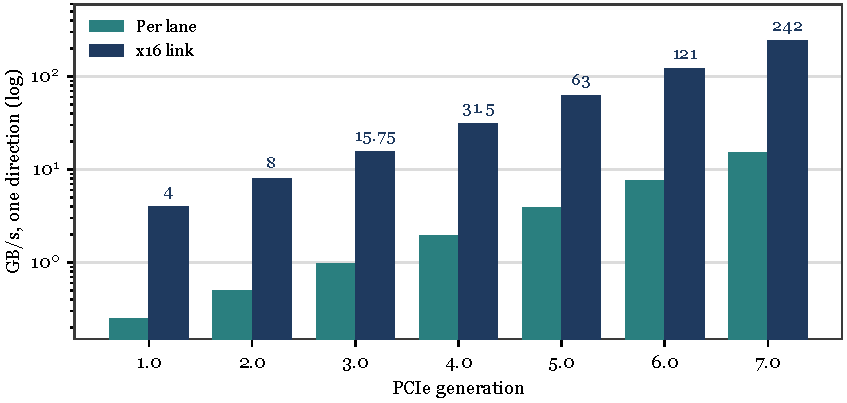
\includegraphics[width=\linewidth]{fig1_link_scaling.pdf}
\caption{PCIe bandwidth by generation, one direction. Per-lane bandwidth has grown sixty-fold while x16 width has not changed; the x16 link reaches 242~GB/s at Gen7, but only by spending more signal integrity per lane.}
\label{fig:scaling}
\end{figure}

\subsection{Four meanings of memory over PCIe}

``Memory bandwidth on PCIe'' describes at least four different traffic patterns: host DRAM read or written by a device over DMA; device memory mapped into the host address space through a BAR; CXL-attached memory that the CPU accesses with loads and stores; and peer-to-peer transfers between two endpoints. They share a physical link but not a protocol path. This paper uses the term for cache-line-granular transfers in any of these patterns, and notes where the DMA path and the load/store path diverge.

\section{The Connector Ration}
\label{sec:connector}

\subsection{Sixty-four data pins}

A PCIe x16 edge connector has 164 contacts, 82 on each side, on a 1.0~mm pitch and an 89~mm card edge \cite{cem}. Only 64 of those contacts are high-speed data pins: 16 transmit pairs and 16 receive pairs. The rest are ground, 12~V and 3.3~V power, the 100~MHz reference clock, PERST\#, WAKE\#, CLKREQ\#, presence detect, JTAG, and SMBus. The connector is therefore not a generic 164-pin interface that happens to carry PCIe; it is a power-and-sideband connector with a data-lane budget attached.

The base specification defines link widths up to x32. The Card Electromechanical specification stops at x16. That gap is the pin ration: an x32 link exists on paper and in some custom ASICs, but not on a standard add-in card. To go wider, a system must use a different connector (SXM, OAM), a cable (CopprLink), or a second slot---each of which gives up compatibility, serviceability, or board area \cite{cem,copprlink}.

\subsection{The connector is a filter}

The connector is also a low-pass filter. At 32~GT/s the Nyquist frequency is 16~GHz. Gen6 does not raise it: PAM4 at 32~GBd keeps Nyquist at 16~GHz, but the modulation's roughly 9.5~dB signal-to-noise penalty makes the same channel behave like a much longer one. Gen7 moves to 64~GBd and 32~GHz. Insertion loss in FR4 rises roughly with the square root of frequency from skin effect and linearly from dielectric loss, and the connector adds pad capacitance, a stub, and crosstalk between adjacent pairs. The result is a loss budget of roughly 30~dB at Nyquist that has not grown across generations. As the rate doubles, the same budget is consumed in half the distance.

Rules of thumb for a conventional PCB stackup put the reach of a Gen3 link near 20 inches, Gen4 near 12, Gen5 near 8, Gen6 near 4, and Gen7 near 2, with wide variation for stackup, connectors, and vias. Beyond that, a retimer is required; it restores the eye but adds a watt, tens of nanoseconds, and cost. The industry's answer for the last two generations has been to leave the board: CopprLink carries 64~GT/s over a copper cable, and PCI-SIG has begun work on optical variants \cite{copprlink}. A cable is a different connector with a different pin budget, which is precisely the point.

\subsection{Power and mechanics}

The slot supplies at most 75~W---5.5~A on 12~V and 3~A on 3.3~V---through the same 164 contacts, and the card is limited to 89~mm of edge and a fixed height. Accelerators that need more use auxiliary cables, which is an admission that the slot's power ration, like its pin ration, was sized for a different era. Power and data share the connector, so a wider data link competes with the power pins for the same edge.

The connector rations three things at once: 64 data pins, about 30~dB of channel, and 75~W. None of the three has scaled with demand, and all three are set by the same mechanical envelope.

\section{The Silicon Ration}
\label{sec:silicon}

\subsection{The SerDes budget}

Each lane is a SerDes: a transmitter with a feed-forward equalizer, a receiver with continuous-time linear equalization and a decision-feedback equalizer, a clock multiplier, ESD structures, and the package and board transitions. In a 7~nm-class process at 32~GT/s, a lane occupies roughly 0.3 to 0.5~mm$^2$ and consumes roughly 3 to 6~pJ per bit, or 100 to 200~mW. A x16 port is therefore 5 to 8~mm$^2$ and 1.5 to 3~W before the controller; at Gen6's 64~GT/s the power roughly doubles. At 121~GB/s, a Gen6 x16 port delivers on the order of 20 to 40~GB/s per watt---respectable, but not free, and energy per bit improves slowly with each node.

\subsection{The root complex budget}

A client processor exposes 16 to 28 lanes; a server socket exposes 64 to 128. Those lanes are shared among graphics, NVMe, Ethernet, CXL, and the chipset link. A 128-lane socket with eight x16 devices has no lanes left for storage or networking, which is why real systems bifurcate slots into x8 and x4 and why lane counts are a marketing specification. The root complex is sized at design time and cannot be expanded in the field; it is a silicon ration that the customer buys as a fixed feature set.

Switches extend the topology but not the budget. A switch adds 100 to 200~ns of latency, one to two watts per port, and cost, and it multiplexes a fixed upstream link across downstream devices, so oversubscription is a bandwidth ration of its own.

\subsection{Beachfront and package}

The physical limit is the die edge. A 600~mm$^2$ die has about 98~mm of perimeter; at 0.5~mm per SerDes lane, that is roughly 200 lanes in total, shared with memory PHYs, Ethernet, and every other high-speed interface. The package imposes a second limit: a x16 link needs on the order of 100 package balls once grounds are counted, plus substrate layers to route them. This is why ``just make it x32'' is not a specification change but a new package, a new board, and a new connector. The one technology that escapes the package edge is 2.5D packaging: an interposer carries HBM's thousand pins a few millimeters, bypassing both the package and the connector. That escape is available to memory, not to a plug-in card.

\subsection{The frequency wall}

Raising the rate is not a free axis either. PAM4 doubles the bits per symbol but costs about 9.5~dB of signal-to-noise ratio relative to NRZ, which must be recovered with equalization, FEC, and a stronger link budget. At 128~GT/s, PAM4 at 64~GBd puts Nyquist at 32~GHz, where conventional FR4 loss is severe and retimers or optics become necessary. SerDes power rises faster than linearly with rate, and the FEC that makes PAM4 reliable adds latency. The physics does not forbid Gen7; it makes Gen7 the point at which copper reach and silicon power become the dominant design constraints.

\begin{table}[t]
\centering
\caption{Constraint budgets for a x16 link. Values are first-order estimates from public specifications and typical implementations; ranges are deliberately wide because they depend on process, stackup, and product class.}
\label{tab:budgets}
\footnotesize
\setlength{\tabcolsep}{4pt}
\renewcommand{\arraystretch}{1.08}
\begin{tabularx}{\linewidth}{@{}>{\raggedright\arraybackslash}p{1.42in}>{\raggedright\arraybackslash}p{1.55in}X@{}}
\toprule
Constraint & Value & Consequence\\
\midrule
Data pins, x16 connector & 64 (32 differential pairs) & 16 lanes maximum on a standard card\\
Link widths, base specification & x1--x32 & x32 exists on paper, not in CEM\\
Connector length / pitch & 89 mm / 1.0 mm & Fixed card edge and contact density\\
Slot power & 75 W & Auxiliary cables for accelerators\\
Channel loss budget & $\sim$30 dB at Nyquist & Reach halves as rate doubles\\
Reach, Gen3 / Gen5 / Gen7 & $\sim$20 / 8 / 2 inches & Retimer or cable beyond reach\\
SerDes area & 0.3--0.5 mm$^2$ per lane & 5--8 mm$^2$ per x16 port\\
SerDes energy & 3--6 pJ/bit & 1.5--3 W (Gen5), 3--6 W (Gen6) per x16\\
Root-complex lanes & 16--28 client, 64--128 server & Shared with all other I/O\\
Die edge, 600 mm$^2$ die & $\sim$98 mm & $\sim$200 lanes total, all interfaces\\
Tag space per function & 32 default / 256 extended & Concurrency ceiling for cache-line traffic\\
\bottomrule
\end{tabularx}
\end{table}

\section{The Transaction Ration: A Latency-Bound Model}
\label{sec:model}

\subsection{The link ceiling}

We model the usable one-directional bandwidth of a link as
\begin{equation}
B_{\mathrm{link}} = R \cdot W \cdot \eta_{\mathrm{enc}} \cdot \eta_{\mathrm{flit}},
\label{eq:link}
\end{equation}
where $R$ is the transfer rate, $W$ the width, $\eta_{\mathrm{enc}}$ the encoding efficiency, and $\eta_{\mathrm{flit}}$ the framing and FEC efficiency. Table~\ref{tab:gens} evaluates this for x16.

\subsection{The protocol ceiling}

A transaction-layer packet carries a header $H$ of roughly 24 bytes once the link-layer sequence and CRC are counted. For a payload $P$, the fraction of link capacity that carries data is
\begin{equation}
\eta_p(P) = \frac{P}{P + H}.
\label{eq:proto}
\end{equation}
Figure~\ref{fig:eff} plots this. At 64 bytes---the size of a cache line and the granularity of a memory read---efficiency is about 73\%. At 256 bytes it is 91\%; at 4~KB it is 99\%. Memory traffic is the worst case for PCIe's header-to-payload ratio, and no amount of signaling improvement changes that.

\begin{figure}[t]
\centering
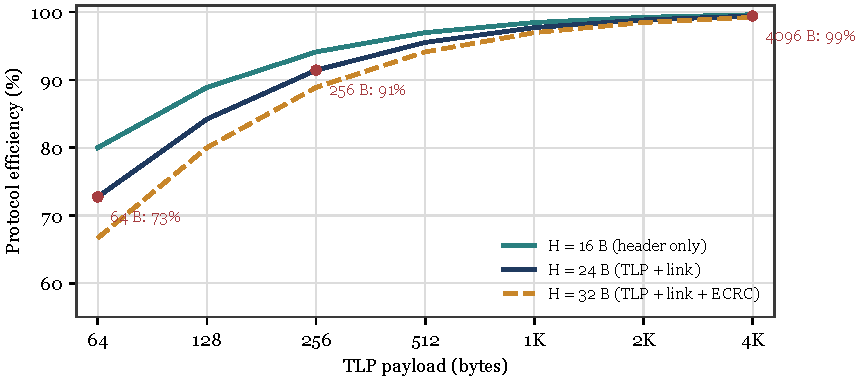
\includegraphics[width=\linewidth]{fig2_efficiency.pdf}
\caption{Protocol efficiency $P/(P+H)$ for three header budgets. Cache-line payloads carry roughly three quarters of the link; the efficiency argument for large DMA transfers is strong, and memory semantics rarely permit them.}
\label{fig:eff}
\end{figure}

\subsection{The concurrency ceiling}

The second term is concurrency. By Little's law, the bandwidth a requester can sustain is $NP/\mathrm{RTT}$, where $N$ is the number of requests in flight and RTT is the round-trip latency. The resulting model is a roofline for the link---the minimum of a rate ceiling and a concurrency ceiling \cite{roofline}---and the two terms combine as
\begin{equation}
B_{\mathrm{eff}} = \min\left( B_{\mathrm{link}}\,\eta_p,\; \frac{N P}{\mathrm{RTT}} \right).
\label{eq:eff}
\end{equation}
RTT on a PCIe memory path is not the pin-to-pin flight time. It includes the root complex, a switch if present, the endpoint's DMA engine and queueing, and the memory controller on the far side. Published CXL and PCIe measurements put the added latency in the hundreds of nanoseconds; for a switchless link, 0.5 to 1~$\mu$s is a reasonable planning number, and 2~$\mu$s is common once a switch and a virtualized endpoint are involved \cite{tpp,pond,directcxl,demystify}.

$N$ is bounded by the Tag field: 32 requests by default, 256 with Extended Tag Enable. Phantom functions can multiply this, and multiple functions or virtual functions each have their own tag space, but a single function on a single link is limited to 256. That is a protocol ration, not a device limitation.

\subsection{What the model predicts}

Table~\ref{tab:requests} evaluates Equation~\ref{eq:eff} for the three most recent generations. At 64-byte payloads and 1~$\mu$s RTT, 256 tags sustain 16.4~GB/s---about a quarter of a Gen5 x16 link and half of a Gen4 x16 link. The default 32 tags sustain 2.05~GB/s. To reach 90\% of Gen5 x16 with 64-byte payloads requires about 886 requests in flight, more than three times the extended tag space of one function. With 4~KB payloads the same link needs only 14 requests, which is why bulk DMA saturates PCIe and cache-line load/store does not.

\begin{table}[t]
\centering
\caption{Requests in flight needed to reach 90\% of the link ceiling, from Equation~\ref{eq:eff}. The last column repeats the calculation for 4~KB payloads; the contrast is the difference between bulk DMA and cache-line memory traffic.}
\label{tab:requests}
\footnotesize
\begin{tabular}{@{}lrrrr@{}}
\toprule
Link (one direction) & $N$, 0.5 $\mu$s & $N$, 1 $\mu$s & $N$, 2 $\mu$s & $N$, 4 KB, 1 $\mu$s\\
\midrule
Gen4 x16, 31.5 GB/s & 222 & 443 & 886 & 7\\
Gen5 x16, 63 GB/s & 443 & 886 & 1,772 & 14\\
Gen6 x16, 121 GB/s & 851 & 1,702 & 3,404 & 27\\
\bottomrule
\end{tabular}
\end{table}

Figure~\ref{fig:latency} makes the regime visible. The latency curves are straight lines on a log-$N$ plot; the link ceilings are horizontal. The intersection is the concurrency needed to saturate the link. Below it, the link is idle; above it, the link is the limit. The tag-space markers at 32 and 256 show how little of the Gen5/Gen6 regime a single function can reach at microsecond latency.

\begin{figure}[t]
\centering
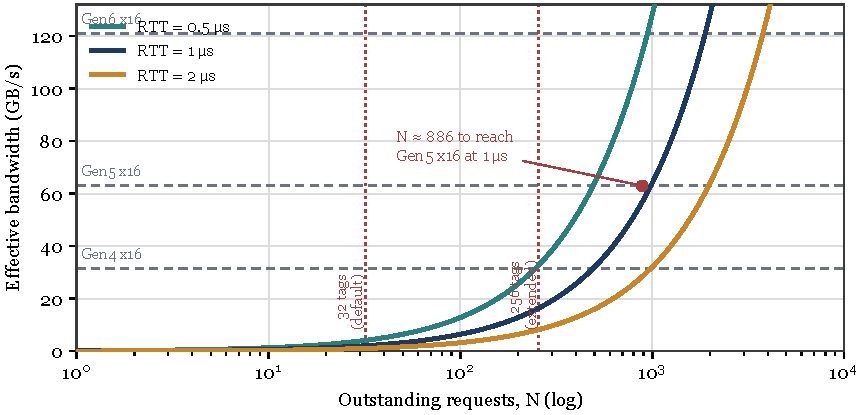
\includegraphics[width=\linewidth]{fig3_latency_bound.pdf}
\caption{Effective bandwidth versus outstanding requests for 64-byte payloads. The dashed horizontals are link ceilings; the dotted verticals are the default and extended tag spaces. A single function cannot reach the Gen5 ceiling at 1~$\mu$s, and cannot come close to Gen6 at any tag depth.}
\label{fig:latency}
\end{figure}

\subsection{Three consequences}

First, a bandwidth number without a payload size, a queue depth, and a latency is not a bandwidth number; it is a link rating. Second, protocols that avoid the DMA bounce, such as CXL.mem, remove one RTT but not the memory latency, so they too need deep queues to approach the link rate. Third, the cheapest way to raise effective memory bandwidth over PCIe is often to raise $P$---coalesce, prefetch, use large DMA transfers---rather than to buy a faster generation.

\section{The Per-Pin Reframing}
\label{sec:perpin}

The usual explanation for the HBM--PCIe gap is that serial signaling is slower than a wide parallel bus. The numbers do not support that explanation. Define the one-directional bandwidth per signal pin, counting a differential pair as two pins. PCIe Gen3 delivers 0.25~GB/s per pin, Gen4 0.49, Gen5 0.99, Gen6 1.89, and Gen7 3.78. HBM2E delivers about 0.45, HBM3 about 0.80, and HBM3E about 1.20. PCIe Gen6 is already faster per pin than HBM3E, and Gen7 is more than three times faster.

\begin{figure}[t]
\centering
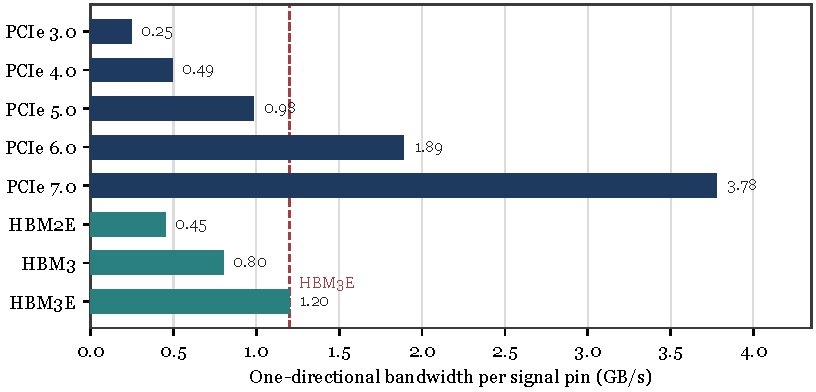
\includegraphics[width=\linewidth]{fig4_per_pin.pdf}
\caption{One-directional bandwidth per signal pin. The crossover is at Gen6: PCIe's problem is not that its pins are slow, but that it has 64 of them and must cross a board. HBM3E's advantage is 1,024 pins and a few millimeters of interposer.}
\label{fig:perpin}
\end{figure}

Figure~\ref{fig:perpin} plots the comparison. The gap is not in the signaling; it is in the number of pins and the distance they span. HBM3E uses 1,024 data pins per stack and a few millimeters of interposer; a PCIe x16 link uses 64 data pins and up to hundreds of millimeters of board. Per pin, PCIe is the faster interface. Per link, it is the pin-poor one.

The comparison has caveats. HBM pins run at lower rate but with lower energy per bit and far lower latency; PCIe pins pay for equalization, FEC, and retimers. The metric ignores duplex asymmetry and the cost of the pins themselves. But it reframes the problem correctly: PCIe is not pin-slow, it is pin-poor. The way to close the gap is to add pins, shorten reach, or both---which is exactly what cables, optics, and advanced packaging do.

\section{Escape Routes}
\label{sec:escape}

\subsection{CXL: keep the pins, change the protocol}

CXL keeps the PCIe physical layer and replaces the transaction layer. CXL.mem carries load/store requests in 64-byte payloads, CXL.cache maintains coherence with the host, and CXL.io is PCIe for discovery and configuration \cite{cxl30,cxl31}. Because the CPU issues loads and stores rather than DMA descriptors, CXL removes the bounce buffer and one round trip, and because CXL 3.0 supports switching and pooling, it separates capacity from the server that uses it.

What CXL does not do is change the pin ration or the reach. A CXL x16 link is a PCIe x16 link at the same rate, over the same connector, with the same channel. Its latency is better than DMA but still hundreds of nanoseconds; published systems report roughly 200 to 400~ns of added latency, which is why the software stack tiers pages rather than treating CXL memory as local DRAM \cite{tpp,pond,directcxl,demystify}. CXL relaxes the transaction ration and the capacity ration. It does not relax the connector or the silicon.

\subsection{NVLink and UALink: spend pins, shorten reach}

NVLink and UALink take the opposite approach: keep the reach short and spend pins. NVLink~5 delivers 1.8~TB/s per GPU over a short copper fabric, and a rack-scale system aggregates it across dozens of GPUs \cite{nvl72,h100}. UALink~1.0 specifies 200~Gb/s per lane for scale-up domains of hundreds of accelerators \cite{ualink}. These links are wider, faster, and more numerous than PCIe, and they are not general-purpose: they connect accelerators to accelerators, not a CPU to a disk.

They relax the pin ration by using many more pins and cables, and they relax the reach ration by keeping runs inside a rack. They do not relax the transaction ration---the memory is still device memory, and the link is still a fabric---but they demonstrate the trade: bandwidth is bought with pins and proximity.

\subsection{Optics: remove the reach term}

Optics relaxes reach directly. A fiber has loss that is nearly flat over the band of interest and is independent of distance up to kilometers, so the channel no longer halves with each generation. Co-packaged optics moves the transceiver next to the ASIC, removing the electrical reach from the die to the module. PCI-SIG's optical work and the copper CopprLink specification are two ends of the same strategy: move the connector off the board \cite{copprlink}.

The costs are real: transceivers consume several picojoules per bit, add latency, and cost more than a copper connector; lasers have reliability and thermal budgets. But optics is the only technology that removes the reach term from the bandwidth equation, which is why rack-scale memory pooling is an optical argument as much as a CXL argument.

\subsection{UCIe: remove the reach entirely}

UCIe goes the other way: instead of extending reach, it removes it. UCIe defines a die-to-die link at 32~GT/s with sub-picojoule per bit energy over millimeters of package routing \cite{ucie}. It is the chiplet equivalent of HBM's interposer: many pins, very short reach, low energy. It relaxes the pin and reach rations at the same time, but only inside a package, and it trades capacity and yield for bandwidth.

HBM is the existence proof. A stack delivers 1.2~TB/s over 1,024 pins and a few millimeters, at energy per bit that no board-level link can match \cite{hbm3e}. The cost is the interposer, the package, and the fact that capacity is fixed at build time.

\subsection{Near-memory compute: reduce demand}

Finally, the cheapest byte is the one that is not moved. Compression, sparsity, in-memory compute, and near-memory accelerators reduce demand rather than increase supply. They are complementary to every mechanism above and, for workloads that can use them, they change the ratio rather than the pipe.

\begin{table}[t]
\centering
\caption{Escape routes and the ration each relaxes. No single mechanism lifts the x16 ceiling; each attacks a different term in the bandwidth equation.}
\label{tab:escape}
\footnotesize
\setlength{\tabcolsep}{4pt}
\renewcommand{\arraystretch}{1.08}
\begin{tabularx}{\linewidth}{@{}>{\raggedright\arraybackslash}p{1.12in}>{\raggedright\arraybackslash}p{1.32in}X>{\raggedright\arraybackslash}p{0.82in}@{}}
\toprule
Mechanism & Ration relaxed & Principal cost & Maturity\\
\midrule
CXL 3.x & Transaction, capacity & 200--400 ns latency; new software stack & Shipping\\
NVLink 5 / UALink & Pins, reach (short) & Proprietary or consortium; scale-up only & Shipping / emerging\\
Optical PCIe / CPO & Reach & Transceiver power, cost, thermals & Emerging\\
UCIe & Pins, reach (mm) & Package cost; capacity fixed at build & Emerging\\
Near-memory compute & Demand & Programmability; limited applicability & Research\\
\bottomrule
\end{tabularx}
\end{table}

\section{Discussion}

The three rations multiply. A link's usable bandwidth is approximately (pins $\times$ rate $\times$ efficiency) divided by a reach penalty, and the memory system's delivered bandwidth is the minimum of that link ceiling and the concurrency bound $NP/\mathrm{RTT}$. The industry's roadmap attacks different terms: Gen6 and Gen7 raise rate, CXL raises efficiency and capacity, NVLink and UALink raise pins, optics and UCIe lower the reach penalty, and near-memory compute lowers demand. No single one of these lifts the x16 ceiling; together they route around it.

The practical lesson is about metrics. A PCIe bandwidth claim should be reported per pin, per watt, and per dollar, with the payload size and queue depth that produced it. The per-pin metric exposes the connector ration; the per-watt metric exposes the SerDes ration; the payload-and-queue disclosure exposes the transaction ration. Without all three, a generation number is a signaling claim, not a system claim.

Two predictions follow, both falsifiable. First, the next significant increase in memory bandwidth at rack scale will come from optical or cabled links and from pooling, not from another doubling of the x16 rate. Second, the connectors that matter will increasingly be cable and fiber connectors, because the edge connector cannot carry more pins and cannot carry them farther. The x16 slot will remain for compatibility, but it will not be where the bandwidth is.

\emph{Threats to validity.} Our model is analytical and first-order; the parameters in Table~\ref{tab:budgets} are estimates from public sources, and vendor specifications are optimistic. We do not measure a real link, and we do not model arbitration, credit stalls, or workload burstiness. The conclusion that the tag space binds is robust to a factor of two in latency; the exact crossover points are not. A calibrated simulation or a measurement campaign on Gen4/Gen5 hardware would be the natural next step.

\section{Conclusion}

PCI Express has spent two decades making a lane faster and no time making a connector wider. The result is a standard that can signal at 128~GT/s but still hands a system sixty-four data pins, a 30~dB channel, and a 75~W slot. On top of that, the transaction layer rations concurrency to 256 outstanding requests per function and efficiency to about three quarters for a cache line. The link rate is the number on the datasheet; the pin count, the reach, and the tag space are the numbers that decide what a system can actually do.

The x16 ceiling is therefore not a failure of signaling. It is a success of signaling that has been asked to compensate for a packaging and protocol design that stopped scaling. The escape routes are already visible: CXL for capacity and protocol efficiency, NVLink and UALink for pins, optics for reach, UCIe and HBM for proximity. The next decade of memory bandwidth will be won by whoever adds the most pins at the shortest reach---not by whoever runs a lane the fastest.

\clearpage
\begin{thebibliography}{19}
\small
\setlength{\itemsep}{1pt}
\setlength{\parsep}{0pt}

\bibitem{pcie6} PCI-SIG, \emph{PCI Express Base Specification, Revision 6.0}, 2022.

\bibitem{pcie7} PCI-SIG, \emph{PCI Express Base Specification, Revision 7.0}, 2025.

\bibitem{cem} PCI-SIG, \emph{PCI Express Card Electromechanical Specification, Revision 5.0}, 2021.

\bibitem{copprlink} PCI-SIG, \emph{CopprLink Specification}, 2024.

\bibitem{cxl30} CXL Consortium, \emph{Compute Express Link Specification, Revision 3.0}, 2022.

\bibitem{cxl31} CXL Consortium, \emph{Compute Express Link Specification, Revision 3.1}, 2023.

\bibitem{wulf} D. Wulf and S. McKee, ``Hitting the memory wall: implications of the obvious,'' \emph{ACM SIGARCH Computer Architecture News}, vol.~23, no.~1, pp.~20--24, 1995.

\bibitem{roofline} S. Williams, A. Waterman, and D. Patterson, ``Roofline: an insightful visual performance model for multicore architectures,'' \emph{Communications of the ACM}, vol.~52, no.~4, pp.~65--76, 2009.

\bibitem{tpp} H. Al Maruf, H. Wang, et al., ``TPP: transparent page placement for CXL-enabled tiered memory,'' in \emph{Proc. ASPLOS}, 2023.

\bibitem{pond} H. Li, D. Berger, et al., ``Pond: CXL-based memory pooling systems for cloud platforms,'' in \emph{Proc. ASPLOS}, 2023.

\bibitem{directcxl} D. Gouk et al., ``DirectCXL: direct access to CXL memory,'' in \emph{Proc. USENIX ATC}, 2022.

\bibitem{demystify} Y. Sun et al., ``Demystifying CXL memory with genuine CXL-ready systems and devices,'' in \emph{Proc. IEEE/ACM MICRO}, 2023.

\bibitem{nvl72} NVIDIA, \emph{NVIDIA GB200 NVL72: A Scalable, Rack-Scale Architecture}, whitepaper, 2024.

\bibitem{h100} NVIDIA, \emph{NVIDIA H100 Tensor Core GPU Architecture}, whitepaper, 2022.

\bibitem{ualink} UALink Consortium, \emph{UALink 1.0 Specification}, 2025.

\bibitem{ucie} UCIe Consortium, \emph{Universal Chiplet Interconnect Express Specification, Revision 1.1}, 2023.

\bibitem{hbm3e} JEDEC, \emph{High Bandwidth Memory 3E (HBM3E) Standard}, 2024.

\bibitem{barroso} L. Barroso, J. Clidaras, and U. H\"olzle, \emph{The Datacenter as a Computer}, 3rd ed., Morgan \& Claypool, 2018.

\bibitem{jouppi} N. Jouppi et al., ``In-datacenter performance analysis of a tensor processing unit,'' in \emph{Proc. ISCA}, 2017.

\end{thebibliography}

\end{document}
